\documentclass[
    11pt,
    a4paper,
    egregdoesnotlikesansseriftitles,
    toc=chapterentrywithdots,
    twoside,openright,
    titlepage,
    parskip=half,
    headings=normal,  % reduces heading size
    listof=totoc,
    bibliography=totoc,
    index=totoc,
    captions=tableheading,  % caption below table
    chapterprefix,
    listof=flat,
    final
]{scrbook}


% details about your thesis
\newcommand{\titel}{Abstractive Text Summarization of Meetings}
\newcommand{\artderarbeit}{Bachelorarbeit}  % {Bachelorarbeit,Masterarbeit}
\newcommand{\autor}{Bastian Oppermann}
\newcommand{\studiengang}{Informatik}  % {Informatik,Wirtschaftsinformatik,Medieninformatik}
\newcommand{\matrikelnr}{3068074}
\newcommand{\erstgutachter}{Prof.\,Dr.~Korbinian Riedhammer}
\newcommand{\zweitgutachter}{Prof.\,Dr.~Ngoc\,Thang\,Vu}
\newcommand{\logo}{figures/TH-Nuernberg-RGB.png}
\newcommand{\keywords}{bert, summarization}
 

% custom head and foot
\usepackage[automark]{scrlayer-scrpage}
\pagestyle{scrheadings}
\ihead{\headmark}
\chead{}
\ohead{\pagemark}
\renewcommand*\chaptermarkformat{\chapappifchapterprefix{\ }% 
  \thechapter.\enskip}

\RedeclareSectionCommand[tocindent=0pt]{section}
\RedeclareSectionCommand[tocindent=0pt]{subsection}
%\RedeclareSectionCommand[tocnumwidth=70pt]{chapter}

\usepackage{scrhack}

% other packages
\usepackage[utf8]{inputenc}
\usepackage[T1]{fontenc}
\usepackage{lmodern,relsize,textcomp,csquotes}
\usepackage{amsmath,amsfonts}
\usepackage[ngerman,english]{babel}  % flip for German thesis
\usepackage[final]{graphicx}
\usepackage{setspace,geometry,xcolor}
\usepackage{makeidx}
\usepackage{paralist,ifthen,todonotes}
\usepackage{url}
\usepackage{pdfpages}

% table setup
\usepackage{longtable}
\usepackage{array}
\usepackage{ragged2e}
\usepackage{lscape}
\usepackage{booktabs}
\usepackage{multirow}

% pdf hyperref
\usepackage[
    bookmarks=true,
    bookmarksopen=true,
    bookmarksnumbered=true,
    bookmarksopenlevel=1,
    pdftitle={\titel},
    pdfauthor={\autor},
    pdfcreator={\autor},
    pdfsubject={\titel},
    pdfkeywords={\keywords},
    pdfpagelabels=true,
    colorlinks=true,
    linkcolor=red,
    urlcolor=magenta,
    anchorcolor=black,
    citecolor=cyan,
    filecolor=magenta,
    menucolor=red,
    plainpages=false,
    hypertexnames=true,
    linktocpage=true,
]{hyperref}
\usepackage[
    nameinlink,
    noabbrev,
]{cleveref} % cleveref, because hyperref has some missing features (e.g. \autoref not being uppercase at the beginning of a sentence) 

% configure your listings style
\usepackage{listings}
\lstset{
	tabsize=3,
	extendedchars=true,
	frame=single,
	showstringspaces=true,
	numbers=left,
	numberstyle=\small,
	breakautoindent=true,
}
\crefname{lstlisting}{listing}{listings}
\Crefname{lstlisting}{Listing}{Listings}

% page setup
% \setlength{\topskip}{\ht\strutbox}
\geometry{paper=a4paper,left=2.5cm,top=3.0cm,bindingoffset=.8cm}
\onehalfspacing
\frenchspacing
\clubpenalty = 10000
\widowpenalty = 10000 
\displaywidowpenalty = 10000

% some commands
\newcommand{\ua}{\mbox{u.\,a.\ }}
\newcommand{\zB}{\mbox{z.\,B.\ }}
\newcommand{\dahe}{\mbox{d.\,h.,\ }}
\newcommand{\bzw}{\mbox{bzw.\ }}
\newcommand{\bzgl}{\mbox{bzgl.\ }}
\newcommand{\eg}{\mbox{e.\,g.}}
\newcommand{\Eg}{\mbox{E.\,g.}}
\newcommand{\ie}{\mbox{i.\,e.}}
\newcommand{\wrt}{\mbox{w.\,r.\,t.\ }}
\newcommand{\etal}{\mbox{\emph{et.\,al.\ }}}


% TODO remove if not needed...
\usepackage{blindtext}


\begin{document}

\setcounter{secnumdepth}{2}  % numerate subsections
\setcounter{tocdepth}{1}  % ...but don't include them in toc

\frontmatter
\thispagestyle{empty}
\pdfbookmark[1]{Cover}{cov}
\begin{titlepage}

\begin{center}


\includegraphics[width=\linewidth]{figures/TH-Nuernberg-RGB.png}\\[1cm]
\LARGE{Fakultät Informatik}\\[2cm]

\huge
\textbf{\titel}\\[1cm]
%
\Large
\artderarbeit~im Studiengang \studiengang\\[1cm]
%
\large
vorgelegt von

\Large
\autor\\[0.5cm]
\small
Matrikelnummer \matrikelnr\\[2cm]

\vspace*{\fill}

\large
\begin{tabular}{p{3cm}p{8cm}}\\
Erstgutachter:  & \quad \erstgutachter\\[1.2ex]
Zweitgutachter: & \quad \zweitgutachter
\end{tabular}
\end{center}

\begin{center}
\copyright\,\the\year
\end{center}

\vspace{-0.5cm}
\singlespacing
\small
\noindent Dieses Werk einschließlich seiner Teile ist \textbf{urheberrechtlich geschützt}.
Jede Verwertung außerhalb der engen Grenzen des Urheberrechtgesetzes ist ohne Zustimmung des Autors unzulässig und strafbar.
Das gilt insbesondere für Vervielfältigungen, Übersetzungen, Mikroverfilmungen sowie die Einspeicherung und Verarbeitung in elektronischen Systemen.

\end{titlepage}
\cleardoublepage

% download the following form and complete it (hit save in your editor)
% https://intern.ohmportal.de/fileadmin/Gelenkte_Doks/Abt/SZS/SB/SB_0050_FO_Pruefungsrechtliche_Erklaerung_und_Erklaerung_zur_Veroeffentlichung_der_Abschlussarbeit_public.pdf
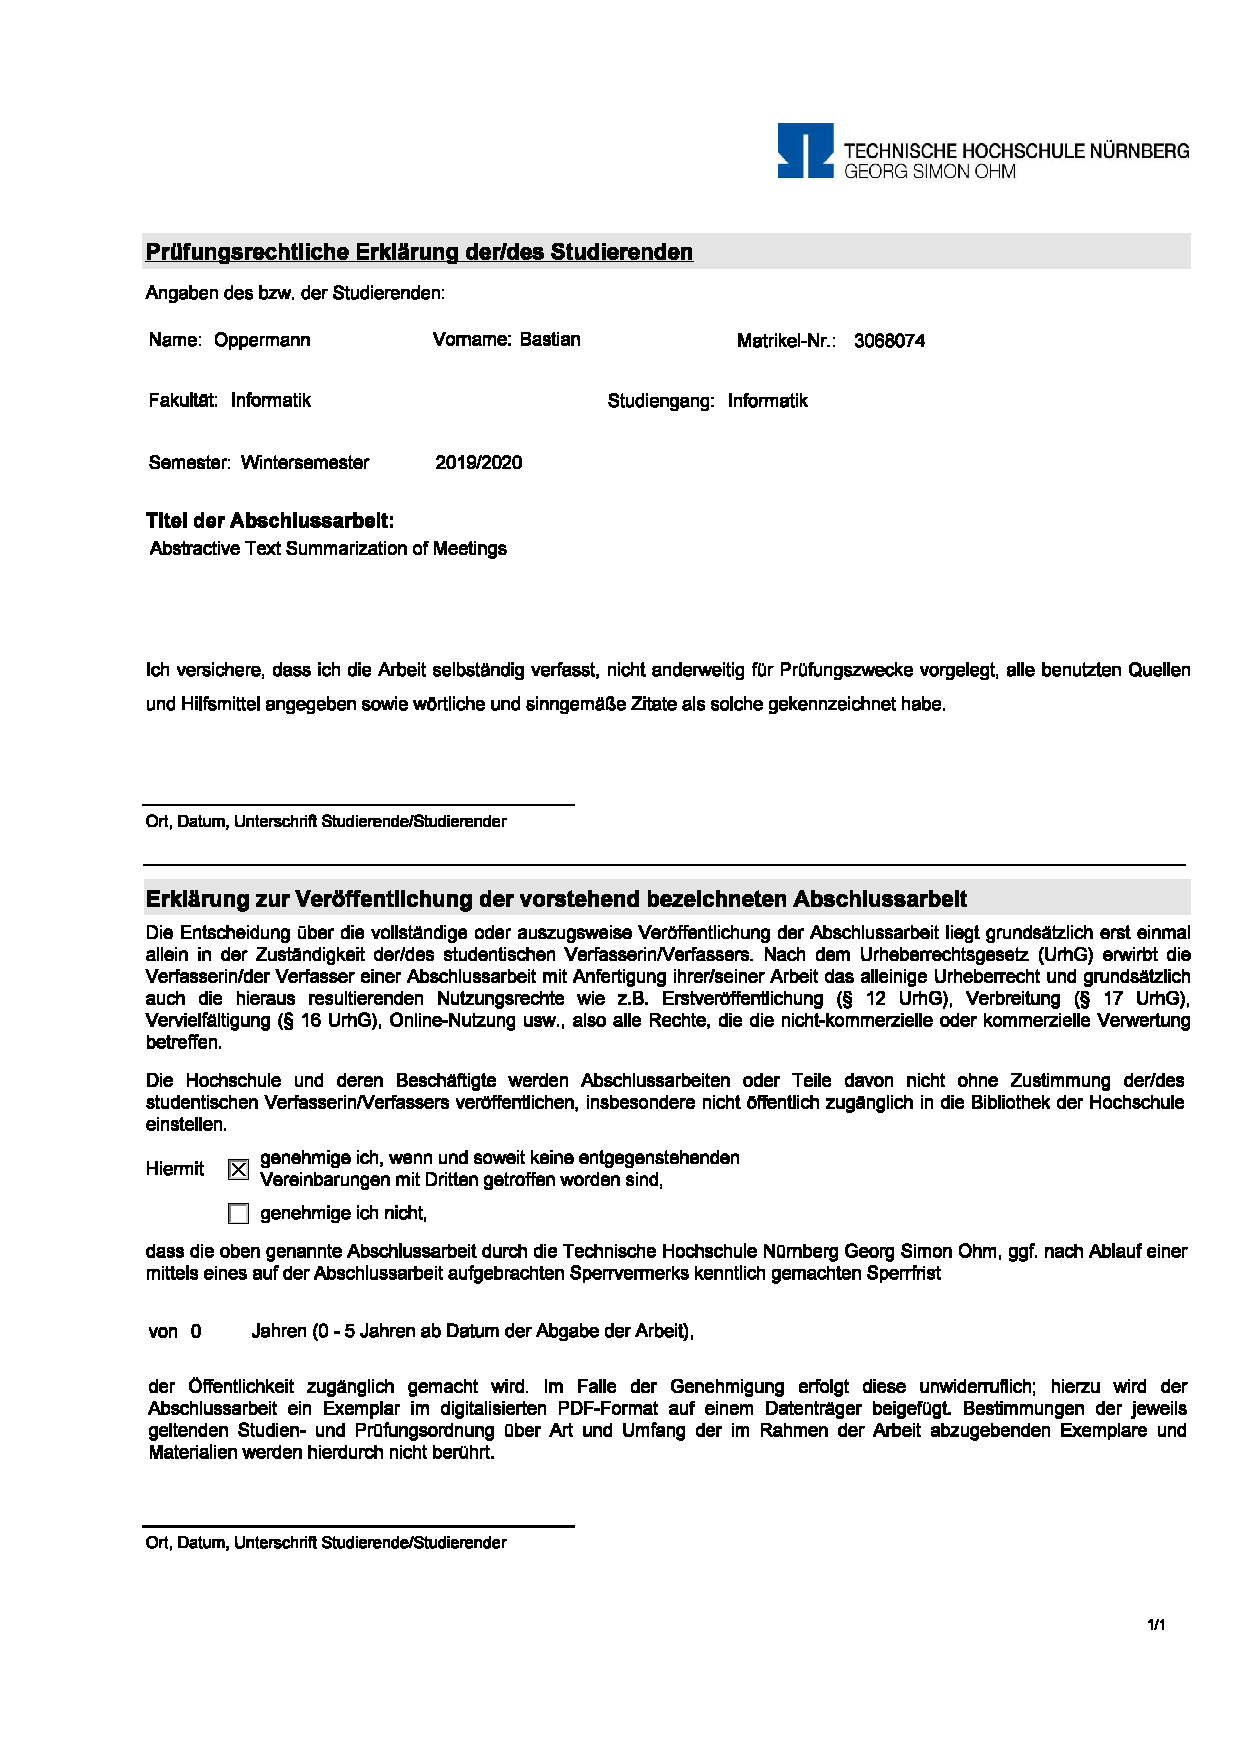
\includepdf{SB_0050_FO_Pruefungsrechtliche_Erklaerung_und_Erklaerung_zur_Veroeffentlichung_der_Abschlussarbeit_public.pdf}\cleardoublepage

\thispagestyle{empty}
\section*{Kurzdarstellung}
\label{sec:kurzdarstellung}

Die vorliegende Bachelorarbeit untersucht, wie ein modernes vortrainiertes neuronales Netz, wie z.B. Googles BERT \cite{devlin2018bert}, zur abstrakten Textzusammenfassung von Meetings genutzt werden kann.

Im Rahmen dieser Arbeit wird ein Tranformer Netz \cite{1706.03762} implementiert, das BERT als seinen Encoder nutzt.
Der Decoder des Netzes ist ein normaler, nicht vortrainierter, Transormer-Decoder.
Das Netz wird hierfür mit Daten aus dem AMI Meeting Corpus \cite{Mccowan05theami} und dem ICSI Meeting Corpus \cite{Janin} trainiert.
Es wird dafür ein 2-stufiges Verfahren genutzt.
Im ersten Schritt wird das Netzwerk darauf trainiert, eine Menge von Dialogen auf einen einzelnen Satz abzubilden, der aus der abstrakten Zusammenfassung des Meetings stammt.
Im zweiten Schritt werden die Meetings nach Themen aufgeteilt und anschließend alle Dialoge eines Themas als Eingabe für das neuronale Netz genutzt.
Die zusammengehängte Ausgabe des Netzes für alle Themen eines Meetings ist dann die fertige Zusammenfassung des gesamten Meetings.
Dies dient zum einen dazu, den benötigten Speicherbedarf von BERT bei langen Textsequenzen zu reduzieren.
Zum anderen kann damit auch das Problem umgangen werden, dass BERT nur mit Textsequenzen bis zu einer Länge von 512 vortrainiert wurde \cite[p.~13]{devlin2018bert}.

Die Arbeit zeigt, dass ein datengetriebener Ansatz in der Theorie funktioniert.
Allerdings haben die Ergebnisse eine sehr starke Neigung dazu, Informationen aus den Traingsdaten in die Zusammenfassung einfliesen zu lassen, selbst wenn diese nicht in der Eingabe vorhanden sind.
Dies ist besonders offensichtlich, wenn ein Netz, das nur mit dem AMI Korpus trainiert wurde, auf den ICSI Corpus angewendet wird.
Die hierbei erziehlten Ergebnisse sind meist sehr schlecht.
Hieraus lässt sich ableiten, dass wesentlich mehr Trainigsdaten notwendig sind, um praxistaugliche Ergebnisse zu erzielen, die unabhängig von einem stark eingegrenzten Kontext, wie es bei den AMI Szenario-Meetings der Fall ist, sind.


\section*{Abstract}
\label{sec:abstract}

This work analyzes how a state-of-the-art pretrained neural network - such as Google's BERT \cite{devlin2018bert} - can be fine-tuned to the task of abstractive text summarization in the context of meetings.

As part of this work a Transformer network \cite{1706.03762} is developed, that uses BERT as its encoder and a plain decoder.
It is trained on the AMI Meeting Corpus \cite{Mccowan05theami} as well as the ICSI Meeting Corpus \cite{Janin}.
To circumvent the high memory usage of BERT at long sequence lengths and the fact that BERT is pre-trained with a maxiumum sequence length of 512 \cite[p.~13]{devlin2018bert}, the summarization is performed using a two-step approach.
First, the network is trained to summarize \(n\) dialouge acts to a single sentence of the meeting's abstractive summary.
Afterwards, a whole meeting is split by its topics and all the dialouge acts of a topic are fed into the trained network as its input.
The concatenated outputs of the Transformer for every topic is the final summary.

The work proofs, that a data-driven approach is feasible in theory.
However, the results have a strong bias towards the context of the meeting and cross-corpus validation on AMI and ICSI shows a very poor performance.
This indicates, that far more training data is necessary for practicable results outside of a very topic-specific context like the scenario meetings of the AMI corpus. \cleardoublepage

\tableofcontents

\mainmatter
\chapter{Introduction}\label{ch:Introduction}

% Motivation

Transfer Learning is known to improve results on many different machine learning tasks.
Google's recently announced language representation model BERT broke records for many Natural Language Processing benchmarks \cite[p.~5--7]{devlin2018bert}, such as  SQuAD v1.1 \cite{rajpurkar-etal-2016-squad} or GLUE \cite{1804.07461}.
There have been some attempts to apply BERT to the problem of abstractive summarization, like \cite{1902.09243} and \cite{1908.08345}.
However, they are usually trained and tested on news articles.
Generating abstractive summaries of meetings is only a rarely researched topic.
Most of the research for summarizing meetings has been focused on either extractive summarization or non Deep Learning approaches such as Dependency Graph Fusion \cite{1609.07035} or Multi-Sentence Compression \cite{shang-etal-2018-unsupervised}.

% ==============
% PROBLEM DEFINITION
% ==============

\section{Problem Definition}

The goal of this work is to analyze, if a data driven approach is feasible for abstractive meeting summarization.
Transfer Learning should be used to compensate for the small amount of training data that is available for meeting summarization.
As BERT's pre-training sequence length of 512 \cite[p.~13]{devlin2018bert} is way shorter than a typical meeting, a method should be developed that deals with this limitation.

% ======
% METHOD
% ======

\section{Method}

As part of this work, a network is developed that uses BERT.
It is trained with data from the two most commonly used meeting corpora, the AMI Meeting Corpus \cite{Mccowan05theami} and the ICSI Meeting Corpus \cite{Janin} that are described in \autoref{ch:used-corpora}.
Cross-corpus validation\footnote{\Eg training on the ICSI corpus and testing on the AMI corpus} is performed to evaluate if the network is able to generalize what it learned.

% =================
% STRUCTURE OF THE WORK
% =================

\section{Structure of the work}

Chapter \ref{ch:theoretical-foundation} explains the theoretical foundation that is necessary for this work.
Chapter \ref{ch:used-corpora} introduces the two used meeting corpora.
Chapter \ref{ch:concept} explains the concept of the model that this works uses.
It will also present how the model is trained.
Chapter \ref{ch:implementation} focuses on the implementation if the model and how the training data is processed.
Chapter \ref{ch:results} presents the results. It shows both the archived scores and provide some hand-picked example outputs.
Chapter \ref{ch:outlook} gives an outlook for possible future research.
Finally, chapter \ref{ch:summary-and-conclusion} summarizes the results of the work and draws a conclusion how they can be interpreted.

\chapter{Data}\label{ch:data}

For this work, two corpora for meeting data are used, the AMI Meeting Corpus \cite{Mccowan05theami} and the ICSI Meeting Corpus \cite{Janin}.

% ==============
% AMI MEETING CORPUS
% ==============

\section{AMI Meeting Corpus}\label{sec:ami-meeting-corpus}

The AMI Meeting Corpus is a corpus for meetings, published by the AMI (Augmented Multi-party Interaction) project in 2006 \cite{Mccowan05theami}.
It contains very detailed annotation of 100 hours of meeting recordings.
The relevant aspects and annotation of the AMI Meeting Corpus, that are relevant for this work, are briefly explained below.

\subsection{Scenario and Non-Scenario Meetings}

The AMI Meeting Corpus contains data for two different types of meetings: Scenario meetings and non-scenario meetings.
For this work, only the data from the scenario meetings are used, as the non-scenario meetings are missing some annotations that are necessary for this work.
The following paragraphs describe the scenario of the scenario meetings.

For the scenario meetings, participants play employees of an electronics company that work together on a project.
They are part of a design team, which tries to develop a prototype for a television remote, because the existing ones are considered not user-friendly, unattractive and old-fashioned.
The participants are assigned one of the following roles:
\begin{itemize}
\item A project manager
\item A marketing expert
\item A user interface designer
\item An industrial designer
\end{itemize}

Each project consists of 4 meetings:
\begin{itemize}
\item A project kick-off meeting
\item A meeting for the functional design of the remote, such as user requirements, technical functionality and the working design
\item A meeting for the conceptual design of the remote's components, such as the materials or the user interface
\item A final meeting to finalize the design and evaluate the results.
\end{itemize}
Before each meetings, the participants perform individual work.

In total, data for 35 of these projects is available, each with the 4 meetings. \cite[p.~2]{Mccowan05theami}

\subsection{Annotations}\label{ssec:ami-annotations}

The following annotations are available and used in this work:

\paragraph{Dialogue Acts}

The transcription of the whole meeting is split into smaller pieces on a per-person basis.
These subsets of the transcription are called "Dialogue Acts".
A dialogue act tries to group word, that belong together to form a speaker's attention, e.g. a question.
Every word of the transcription is part of exactly one dialogue act.
Each dialogue act is classified by its content, but this classification is not used in this work. \cite{amiWebsite}

\paragraph{Topic Segmentation}

Each meeting is split into multiple topics that by themselves may be split into subtopics.
Examples for topics are "industrial designer presentation", "evaluation of prototype" or "project specs and roles of
participants" to name a few. \cite{amiWebsite}

\paragraph{Abstractive Summaries}

\begin{figure}[h]
\begin{lstlisting}[numbers=none]
S1: The project manager introduced the upcoming project to the 
    team members and then the team members participated in an
    exercise in which they drew their favorite animal and
    discussed what they liked about the animal.
S2: The project manager talked about the project finances and
    selling prices.
S3: The team then discussed various features to consider in making
    the remote.
\end{lstlisting}
\caption{Example abstract of abstractive summary for scenario meeting \texttt{ES2002a}.}
\label{fig:abstractive-summary-example}
\end{figure}

For each meeting, abstractive summaries are available.
Each abstractive summary consists of an abstract, decisions, problems/issues and actions, but this work is only using the abstract.
Usually, the abstract consists of multiple sentences.
An example for such an abstract with 3 sentences is shown in \cref{fig:abstractive-summary-example}.

Additionally, for each sentence of the abstractive summary, one or more dialogue acts are selected, that are linked together.
This mapping of $n$ dialogue acts to $1$ sentence of the summary is later used for training, as described in \label{sec:concept-training} in more detail. \cite{amiWebsite}

\subsection{Segmentation of the Corpus}\label{ssec:ami-segmentation-of-the-corpus}

\begin{table}[h]
\centering
\begin{tabular}{@{}ll@{}}
\toprule
\multicolumn{1}{c}{Set} & \multicolumn{1}{c}{Time} \\ \midrule
Training & $\sim$50 hours \\
Development & $\sim$11 hours \\
Test & $\sim$11 hours \\ \bottomrule
\end{tabular}
\caption[Distribution of meeting time of train, dev and test sets]{Distribution of meeting time of train, dev and test sets \cite{amiWebsite}.}
\label{tab:meeting-time-distribution}
\end{table}

To make results comparable with other works that use the corpus, it is split into training, development and test sets.
For the scenario meetings, the data distribution is shown in \cref{tab:meeting-time-distribution}. \cite{amiWebsite}

% ==============
% ICSI MEETING CORPUS
% ==============

\section{ICSI Meeting Corpus}

The ICSI Meeting Corpus, that contains meetings that were collected at the International Computer Science Institute (ICSI) over a period of three years.
It contains about 72 hours of meeting data. \cite{Janin}
As it has a very similar structure than the AMI Meeting corpus described in \cref{sec:ami-meeting-corpus}, this chapter will only focus on their differences that are relevant for this work.

\paragraph{Scenario}

Unlike the scenario meetings of the AMI Meeting Corpus, the ICSI Meeting Corpus are natural meetings that do not have a specific topic.
However, as the meetings are all recorded at the ICSI, they usually follow a specific type.
Because of this, every meeting of the corpus is classified as on one of 5 different meeting types. \cite{Janin}
% TODO Maybe name/describe the 5 types of meetings. But as they are not really important, I will omit them for now...

\paragraph{Topic Segmentation Annotation}

For ICSI, only automatic topic segmentation is available, but no manual segmentation like for AMI.

\paragraph{Segmentation of the Corpus}

Unlike the AMI corpus, the ICSI Meeting Corpus does not come with a predefined split for training, development and test sets.
Because of this missing split, this work will mainly work with the AMI Meeting Corpus and only use the ICSI Meeting Corpus for cross-corpus-validation.
\chapter{Theoretical Foundations}\label{ch:theoretical-foundations}

% ===============
% LEARNING FROM DATA
% ===============

\section{Learning from Data}

\subsection{Labeled and Unlabeled Data}

When learning from data, it is usually either labeled or unlabeled.
An example of labeled data can be images with a caption, where the image itself is the data and the caption is the label.
For abstractive summarization tasks, data is usually labeled with the source text being the data and the summary of this text being the label.
Unlabeled data can be any data, such as plain images or texts.
Unlike labeled data, the amount of unlabeled data is usually much higher as labeling data is an expensive manual process, while unlabeled data is usually produced as a by-product.
A popular example of unlabeled text data is Wikipedia, which contains over a billion words in English alone \cite{wikipediaStats}. 

%TODO Source?

\subsection{Neural Networks}

\begin{figure}[h]
\centering
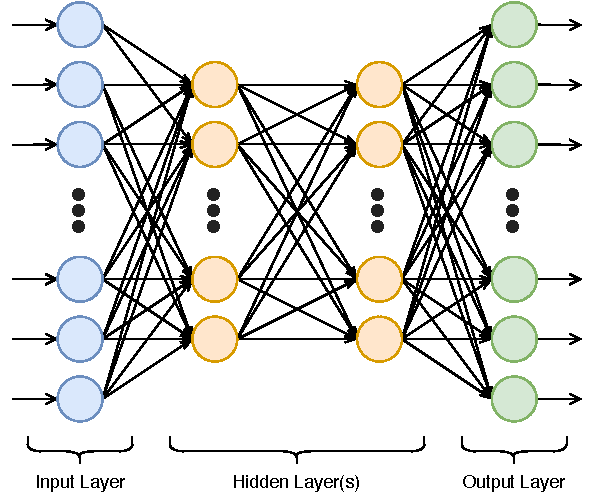
\includegraphics[width=0.45\paperwidth]{figures/neural-network}
\caption{Simple feed-forward neural network with two hidden layers}
\label{fig:neural-network}
\end{figure}

Artificial neural networks are currently a popular and common way to learn from data due to the availability of better hardware and an increasing amount of training data.
A typical neural network consists of neurons that are inspired by real brain neurons and connections between these neurons.
Each neuron can be seen as a function that takes the values of all its predecessor nodes as input and outputs a value that, by itself, is used as the input for its successor nodes.
To compute a node's output, the value $x \in X$ of every predecessor node is multiplied with a weight $w \in W$.
Then, a constant bias, $b$, is added to the sum of these multiplications, and finally an activation function $\Phi$ is applied to this sum as shown in the following equation:
\[
	y = \Phi(\sum_{i=0}^{d}x_iw_i + b)
\]
with $d$ being the number of predecessor nodes and $y$ being the node's output.
For most nodes, the activation function $\Phi$ is usually a nonlinear function that maps its input to values between $-1$ and $1$ or $0$ and $1$.
A popular example of an activation function is sigmoid, which maps negative values to values close to $0$ and positive values to values close to $1$ \cite[p.~4--13]{Aggarwal2018}.

\paragraph{Feed-Forward Networks}

One of the simplest and most common neural network architectures is the feed-forward network.
Such a network consists of multiple layers, where neurons only have predecessors in the previous layer and successors in the next layer.
The first layer with no predecessors is called the input layer as here the actual input for the neural network is used as the node's values.
The last layer with no successors is called the output layer.
The values of the nodes in the output layer are used as the output of the whole network.
Every layer in between these two layers is called a hidden layer.
While the nodes in the hidden layer usually have a nonlinear activation function, nodes in the output layer sometimes have a linear activation function like ReLU if the output is an absolute value. 
Such a network is shown in \cref{fig:neural-network} \cite[p.~17--20]{Aggarwal2018}.

\paragraph{Backpropagation}

When training a network, the goal is to adjust all the weights and biases in a way that the error of the neural network is minimized.
This error is measured with a loss function that computes how different the output of the network for the training data is compared to the desired output (the labels).
Backpropagation is an algorithm that computes how the weights and biases should be adjusted.
The backpropagation algorithm consists of two phases: In the forward phase, a portion (batch) of the training data is fed into the network, and the loss is computed.
In the backward phase, the gradients of the loss function are computed, and then these gradients are used to update the weights of the network.
This processes is repeated multiple times \cite[p.~21--24]{Aggarwal2018}.

% TODO Maybe add an "Overfitting" paragraph

\subsection{Automatic Evaluation}\label{ssec:automatic-evaluation}

Evaluating summaries is essential for multiple reasons (\eg, to monitor progress during training or to compare own results to results from other researchers).
While human evaluation seems like an obvious approach, it is usually not feasible because it is slow and expensive, and results from different people are not always comparable.
Thus, the more common approach is automatic evaluation.
To automatically evaluate summaries, Recall-Oriented Understudy for Gisting Evaluation (ROUGE) \cite{lin-2004-rouge} is widely adapted as it tends to correlate well with human judgments.
In addition, ROUGE supports multiple evaluation metrics.
To report the results achieved in this thesis, the following three metrics are used:
\begin{itemize}
\item \textbf{ROUGE-1}, which calculates the overlap of single words (unigrams) between the candidate summary and the reference summary
\item \textbf{ROUGE-2}, which is similar to ROUGE-1, but instead of using the overlap of single words, it uses word pairs of two (bigrams)
\item \textbf{ROUGE-L}, which uses the longest common subsequence to calculate the score. A subsequence must not be confused with a substring. For the sentences "My favorite name is John Doe" and "My name is Maria Doe," the longest common subsequence would be "My name is Doe," whereas the longest substring would just be "name is."
\end{itemize}

When comparing word overlap, one must differentiate between recall and precision \cite{Ting2010}.
While recall indicates how much information of the reference summary is present in the candidate summary, precision indicates how much of the information in the candidate summary is actually present in the reference summary.
It is common to combine these two measures to a single one, called F1-measure.
It is calculated by the following formula:
\[
	F_1 = 2 \cdot \frac{Recall \cdot Precision}{Recall + Precision}
\]

% ==========
% TRANSFORMER
% ==========

\section{Transformer}\label{sec:transformer}

The Transformer is a neural network architecture for sequence learning that was published in 2017 \cite{1706.03762}.
It achieved new state-of-the-art results for many machine translation tasks while at the same time requiring significantly less training time compared to previous well-performing models.

\subsection{Motivation}\label{ssec:transformer-motivation}

In recent years, recurrent neural networks (RNNs) have been the most common way to solve sequence learning tasks.
However, one of the major downsides of RNNs is their sequential behavior.
To train an RNN, the elements of the input sequence are fed into the neural network one after another.
While the sequence elements are passed through the RNN, a hidden state gets computed at every step, which is part of the input for the next step.
This process is called encoding.
Afterward, the last hidden state of the encoding process is used as an input for the first step of the decoding process.
Because of this, it is not possible to parallelize the training within a training example as the hidden state of the previous step is needed to calculate the output of the current step \cite[p.~2]{1706.03762}.
A simplified RNN for sequence-to-sequence tasks like machine translation is shown in \cref{fig:rnn-visualization}.

\begin{figure}[h]
\centering
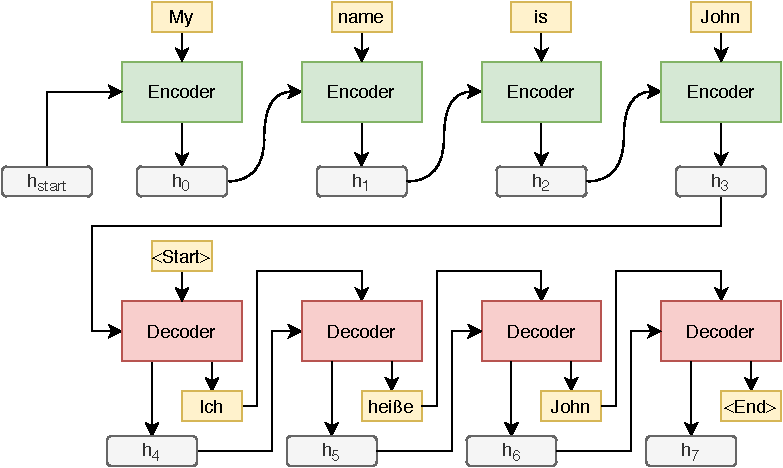
\includegraphics{figures/rnn-visualization}
\caption[Simplified visualization of a sequence-to-sequence RNN network for machine translation]{Simplified visualization of a sequence-to-sequence RNN network for machine translation. The input sequence is fed into the encoder with one word for each step. The final hidden state, which is computed in the last encoding step, is used as input for the first decoding step. The initial hidden state, $h_{start}$, can be initialized as a vector of zeros or learned during training.}
\label{fig:rnn-visualization}
\end{figure}

Another problem with RNNs is the long distance, that information must "travel" before it is used. % TODO Illustrate this long "travel" distance
Information that was encoded into the hidden state must pass through multiple encoding and decoding steps, before it is finally used in one of the decoding steps.
Besides having the hidden state as an information bottleneck, this also makes it very hard for the network to learn long range dependencies because of the problem of vanishing or exploding gradients \cite{Hochreiter01gradientflow}. % TODO Maybe briefly explain the problem
Modern variants of RNNs, like the long short-term memory (LSTM) architecture \cite{Hochreiter1997}, try to mitigate these effects but are not able to fully eliminate them.
A fairly recent solution to this problem is the attention mechanism that was first proposed in 2014 \cite{1409.0473}.
It allows the network in the decoding stage to retrieve information from any hidden state that was computed during the encoding stage.
This eliminates the issue of learning long range dependencies.

The Transformer network takes advantage of the attention mechanism while avoiding the recurrence of RNNs to achieve faster training and allow for more parallelization.

\subsection{Model Architecture}\label{ssec:transformer-model-architecture}

Just like sequence-to-sequence RNNs, the Transformer consists of an encoder and a decoder that both have multiple stacks of layers.

\begin{figure}[h]
\centering
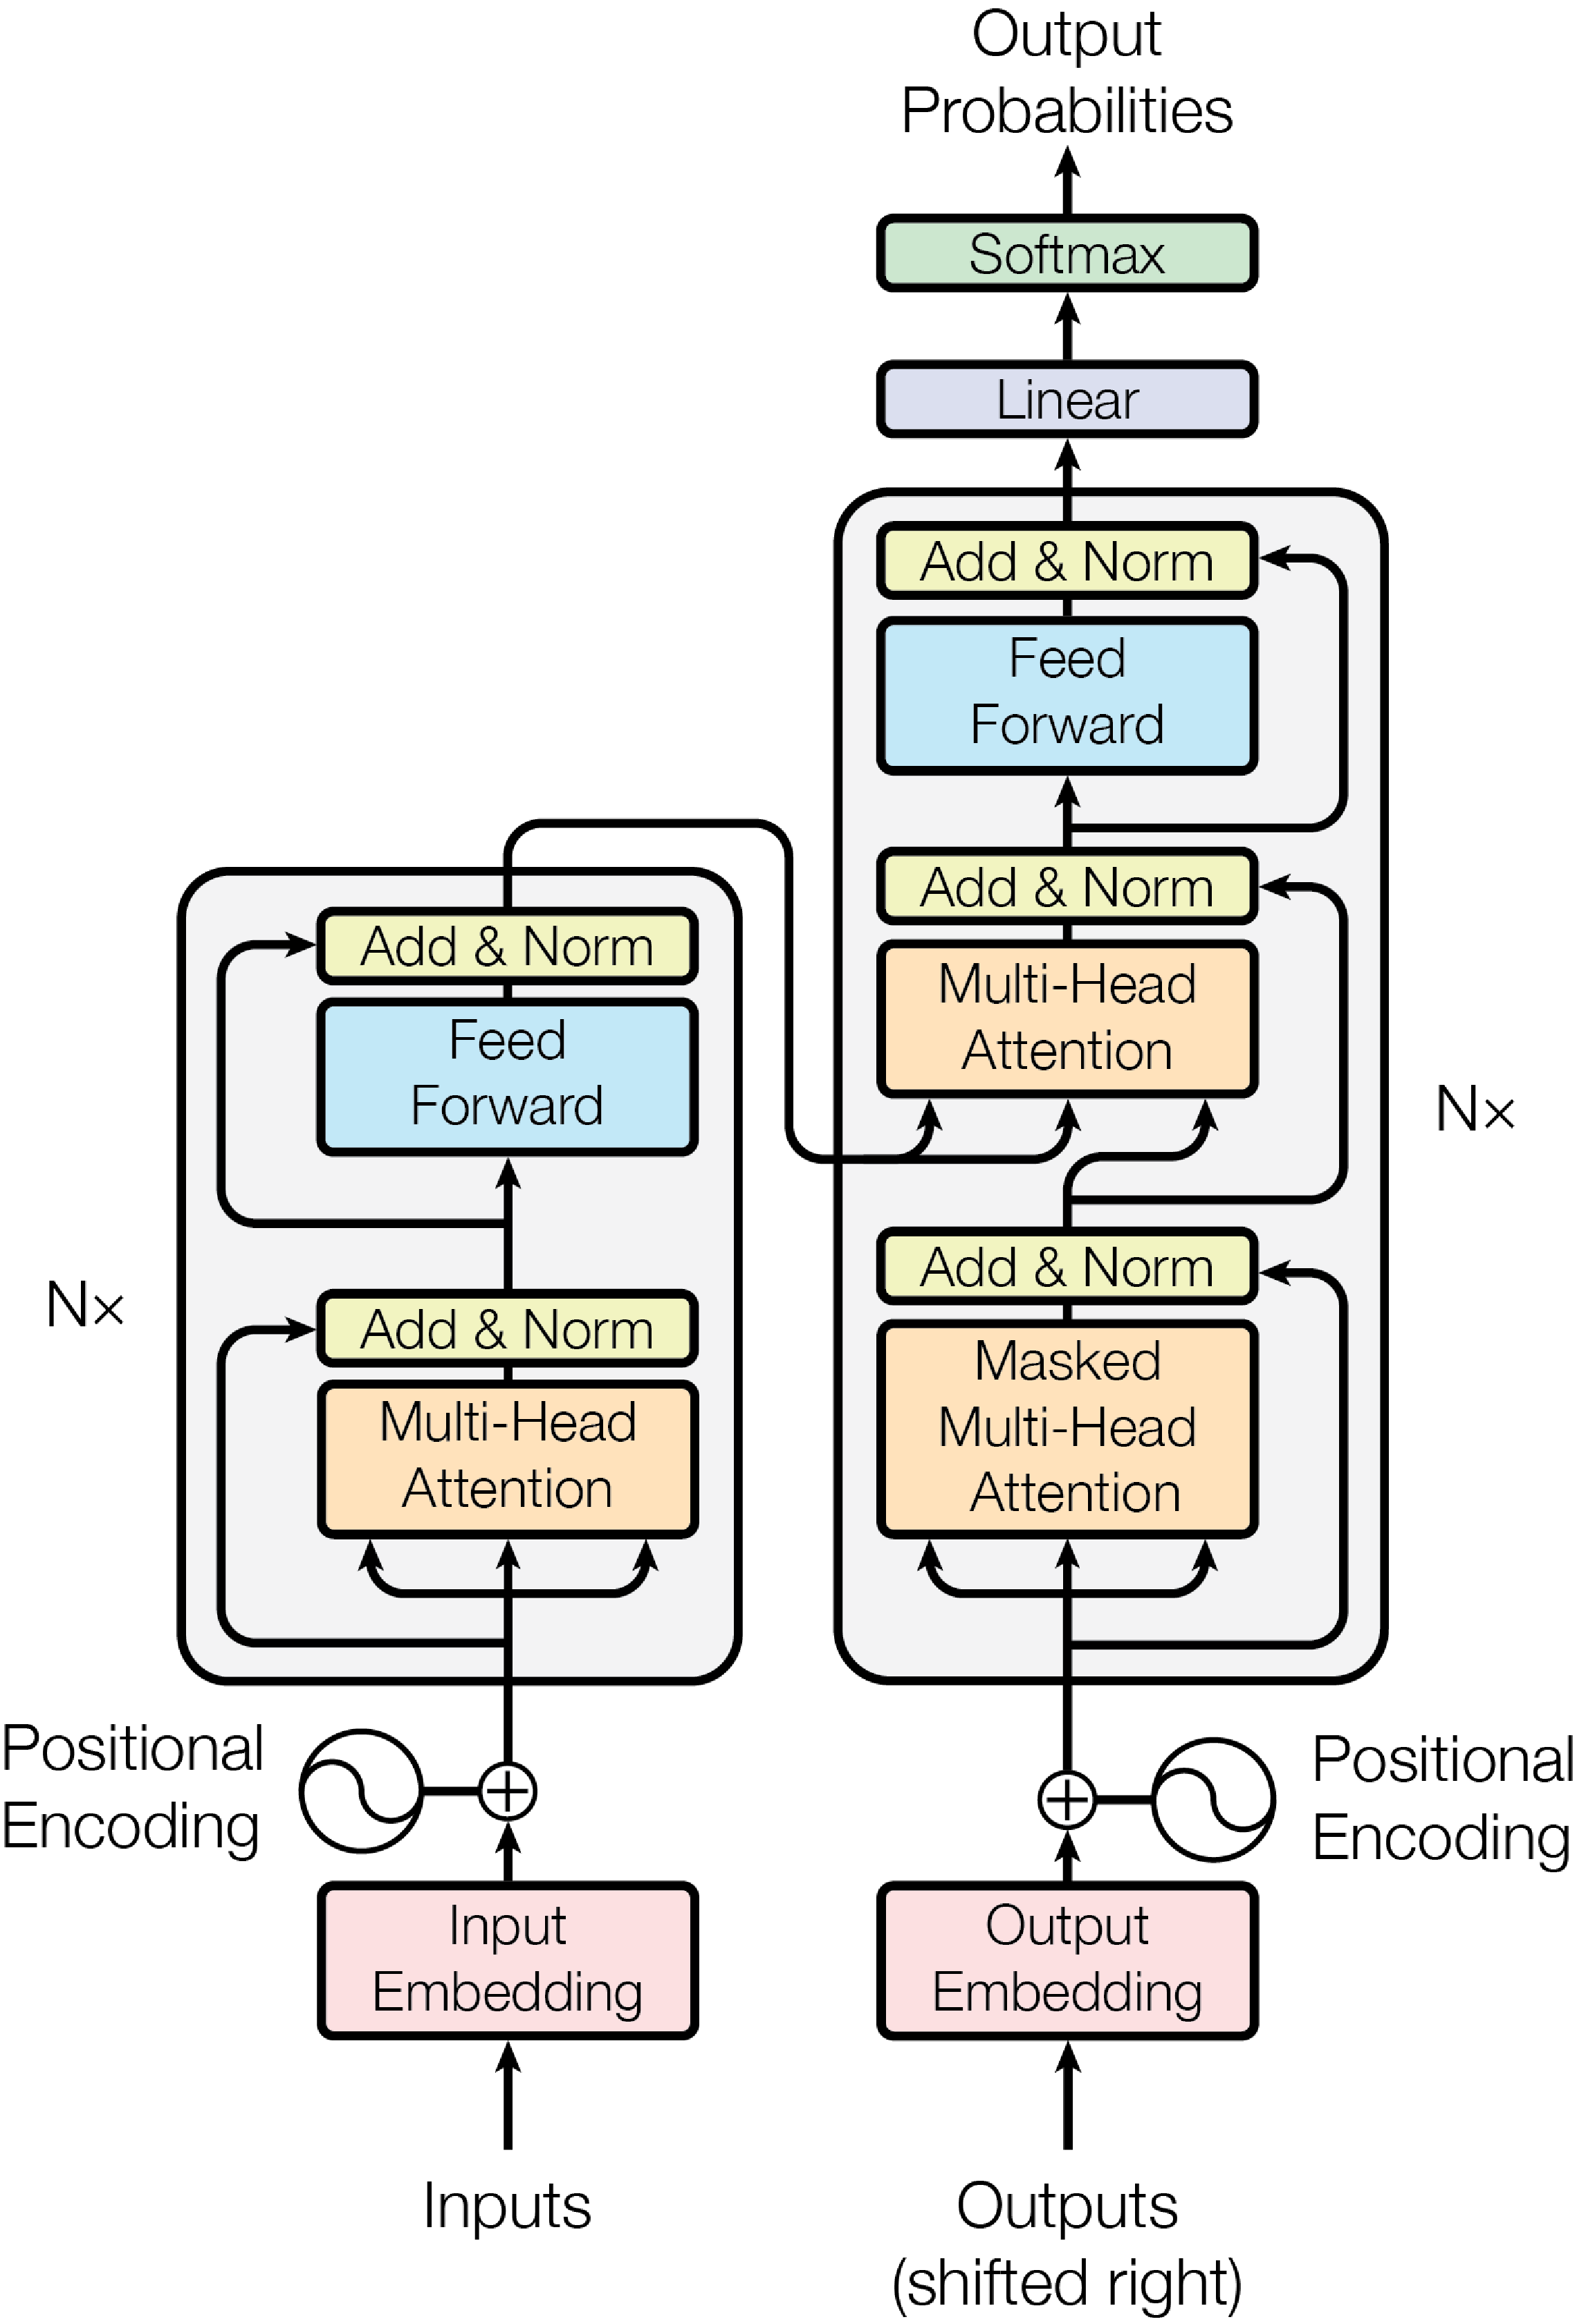
\includegraphics{figures/transformer-model}
\caption[Model architecture of a Transformer]{Model architecture of a Transformer \cite[p.~3]{1706.03762}}
\label{fig:transformer-model}
\end{figure}

An encoder layer consists of two sublayers.
The first sublayer is a multi-head self-attention mechanism, which is described later in this section.
The second sublayer is a position-wise\footnote{The identical network is applied to each position separately \cite[p.~5]{1706.03762}.} fully connected feed-forward network.
Both sublayers have residual connections \cite{1512.03385} around them that are followed by layer normalization \cite{1607.06450}.
The outputs of the layers of the Transformer base model have $d_{model}=512$ dimensions and $d_{model}=1024$ for the big model \cite[p.~9]{1706.03762}.

An encoder layer has a similar structure but with one additional sublayer and a slight modification of the multi-head self-attention sublayer.
The new sublayer attends to the output of the encoder.
The multi-head self-attention sublayer is masked to prevent it from attending to future words \cite[p.~3]{1706.03762}.

In the original Transformer, $N = 6$ stacked encoder and decoder layers are used for both the base and the big model.
The complete architecture of the Transformer is visualized in \cref{fig:transformer-model}.

The inputs are simple learned embedding vectors of dimension $d_{model}$ that are concatenated with a fixed positional embedding \cite[p.~5--6]{1706.03762}.
These fixed input embeddings encode the position of the sequence elements as this information is otherwise no longer accessible to the network because of the missing recurrence.
The positional encoding is calculated with sine and cosine functions of different frequencies:
\begin{align*} 
	PE_{(pos,2i)} & = sin(pos/10000^{2i/d_{model}}) \\
	PE_{(pos,2i+1)} & = cos(pos/10000^{2i/d_{model}})
\end{align*}

This encoding allows the network to obtain information about the absolute and relative position of each element.
\Cref{fig:positional-encoding-sine-cosine} illustrates the embedding for some dimensions.
It is clearly visible how each position has a different positional embedding.

For the outputs, a learned linear transformation and a softmax function are used to compute next-token probabilities \cite[p.~5]{1706.03762}.

\begin{figure}[h]
\centering
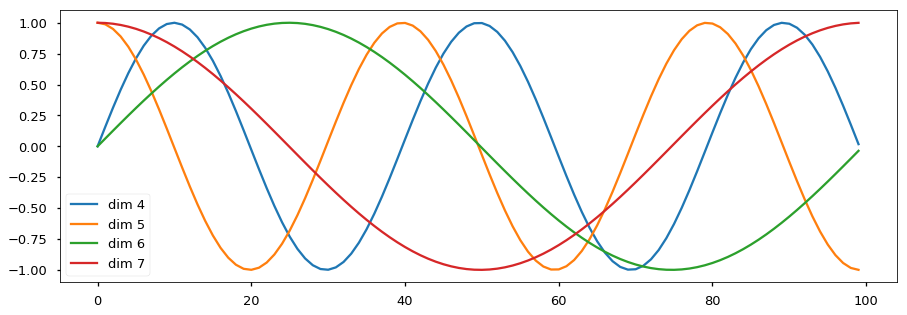
\includegraphics[width=0.7\paperwidth]{figures/positional-encoding-sine-cosine}
\caption[Visualization of positional encoding with sine and cosine]{Visualization of positional encoding with sine and cosine \cite{annotated.transformer}}
\label{fig:positional-encoding-sine-cosine}
\end{figure}

\paragraph{Attention}

\begin{figure}[h]
\centering
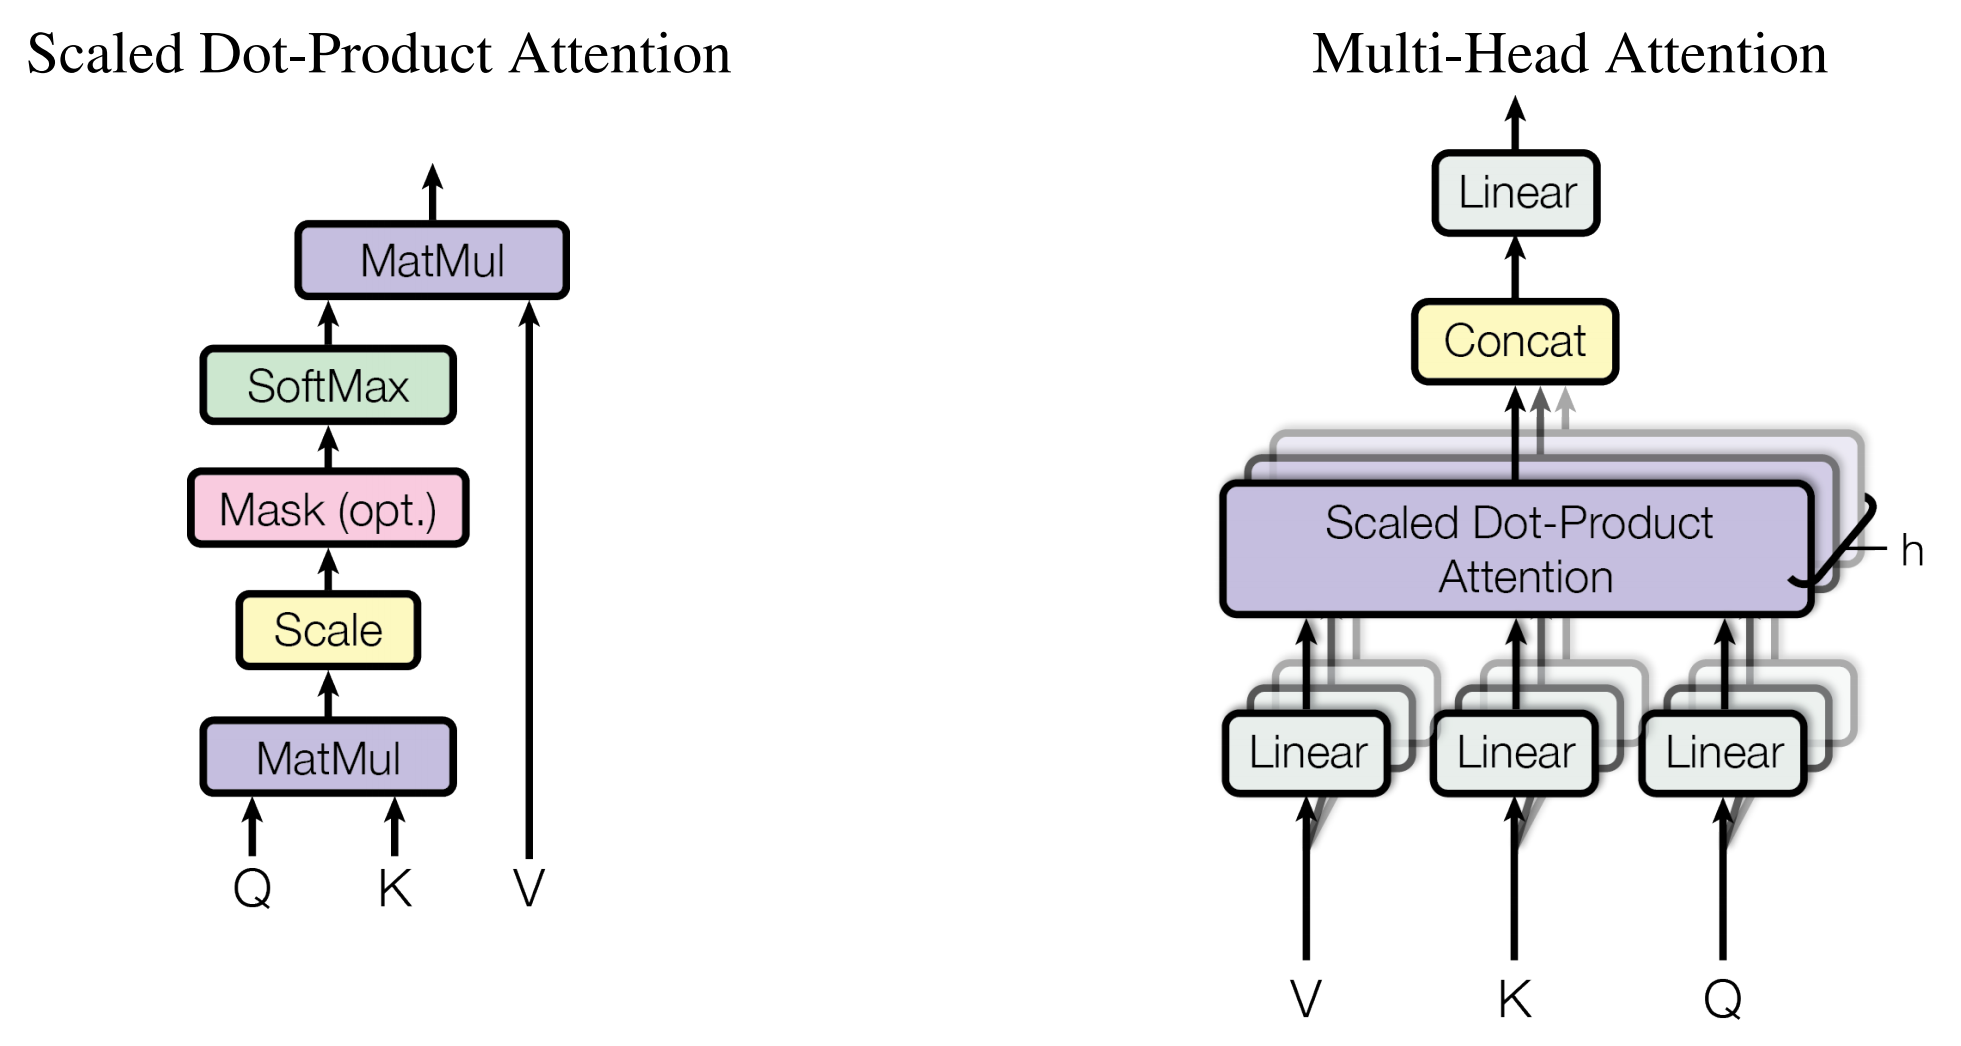
\includegraphics[width=0.7\paperwidth]{figures/scaled-dot-product-multihead-attention}
\caption[Visualization of scaled dot-product attention and multi-mead attention]{Visualization of scaled dot-product attention and multi-head attention \cite[p.~4]{1706.03762}}
\label{fig:scaled-dot-product-multihead-attention}
\end{figure}

The Transformer attention consists of query, key, and value vectors.
The query vectors are used to select values by their corresponding keys.
The Transformer implements this as a scaled dot-product attention, wherein queries and keys have the dimension $d_k$ and the values the dimension $d_v$.
To calculate the attention, the following formula is used:
\[
	\textrm{Attention}(Q,K,V) = \textrm{softmax}(\dfrac{QK^T}{\sqrt{d_k}})V
\]
where $Q$, $K$, and $V$ are matrices that contain multiple sets of queries, keys, and values \cite[p.~3--4]{1706.03762}.
Masking for the decoder layer is easily performed by setting the input values of the softmax function to $-\infty$ if they are not allowed.

Unlike normal attention, the Transformer uses multi-head attention.
This means that instead of having a single attention function, the queries, keys, and values are linearly projected with learned linear projections \cite[p.~4--5]{1706.03762}.
After performing the attention function on the projected matrices, they are concatenated and projected again.
The dimension of each learned linear projection is the model's dimension $d_{model}$ divided by the number of attention layers $h$.
\Cref{fig:scaled-dot-product-multihead-attention} shows both the scaled dot-product attention (left) and the multi-head attention (right).

\subsection{Advantages}

As described in \cref{ssec:transformer-motivation}, the Transformer allows for significantly more parallelization than RNNs because of the absence of sequential behavior within one training example.
This yields much faster and less expensive training compared to previous state-of-the-art models for machine translation.
The big Transformer model is trained for 3.5 days on 8 P100 GPUs and the base Transformer model for just 12 hours \cite[p.~7]{1706.03762}. 
In comparison, the first RNN network to utilize attention took between 109 and 252 hours for training \cite[p.~14]{1409.0473}.

\subsection{Disadvantages}

Transformer networks tend to get very large and require a large amount of memory, especially for longer sequence lengths as the self-attention connects every position with every other position in the sequence.
This results in quadratic complexity for the sequence length.
As a solution, the authors of the Transformer suggest limiting the self-attention to the neighbors of each position \cite[p.~6--7]{1706.03762}.  
The more recent Reformer \cite{kitaev2020reformer} solves this issue by using locality-sensitive hashing to reduce the complexity from $O(L^2)$ to $O(L)$.

% ====
% BERT
% ====

\section{BERT}\label{sec:bert}

Bidirectional Encoder Representations from Transformers (BERT) is a general-purpose language model that was released by Google AI researchers in mid-2018.
It broke several records for natural language processing benchmarks \cite[p.~5--7]{devlin2018bert}, such as  SQuAD v1.1 \cite{rajpurkar-etal-2016-squad} and GLUE \cite{1804.07461}.

\subsection{Motivation}

It has been shown that results for many natural language processing tasks can be improved with the help of language models.
The most famous among them are OpenAI's GPT-2 \cite{radford2019language} and ELMo \cite{1802.05365}.
The benefit of language models is that most of them can be trained on unlabeled data like Wikipedia articles or large book corpora.
This allows them to learn from a huge amount of data as there is no need for time-consuming labeling of the training data and any texts can be used.
By pretraining them on normal texts, the networks can get a general sense of natural language, which can then be used for more specific tasks.

% TODO Not sure if I keep using this or create an own one / just remove it
\begin{figure}[h]
\centering
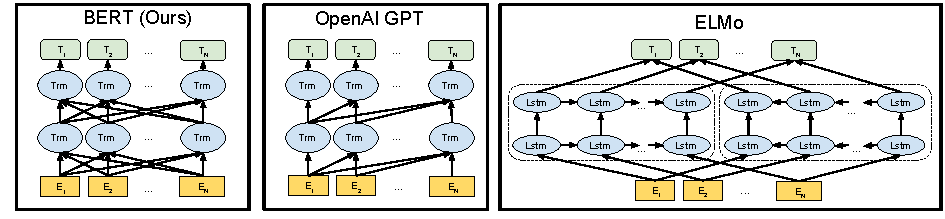
\includegraphics[width=0.7\paperwidth]{figures/bert-gpt2-elmo-model-comparison}
\caption[Visualization of the different model architectures]{Visualization of the different model architectures \cite[p.~13]{devlin2018bert}}
\label{fig:bert-gpt2-elmo-model-comparison}
\end{figure}

What is new about BERT compared to other models like GPT-2 is that it is the first deeply bidirectional language model that takes advantage of the whole context around a word.
OpenAI's GPT-2 uses a left-to-right Transformer decoder \cite[p.~4]{radford2019language}, which only allows it to "look" at the words to the left when generating a representation for an input token.
For example, with a sentence that starts with "The lighter," the network can only look at these two words to generate a representation for the word "lighter."
However, the word can have completely different meanings depending on the whole sentence (\eg, "The lighter is an easy tool for making fire" compared to "The lighter shade of red looks better than the darker one"). 
ELMo compensates for this issue by training two LSTMs, one being a normal forward LSTM (left-to-right) and the other one being a backward LSTM (right-to-left), which is given the input sequence in reverse \cite[p.~2--3]{1802.05365}.
Afterward, it concatenates the representations of these two LSTMs to get a semi-bidirectional representation.
\Cref{fig:bert-gpt2-elmo-model-comparison} presents the different architectures.

\subsection{Model Architecture}

At its core, BERT is just a Transformer encoder, as described in \cref{ssec:transformer-model-architecture}.
What is innovative about BERT's architecture is mainly how it is trained and how the inputs and outputs are represented.

\paragraph{Input and Output Representations}

BERT's input is applicable to many different natural language processing tasks.
It allows the inputs of either one sentence or a pair of two sentences.\footnote{In the context of BERT, a sentence does not refer to an actual linguistic sentence, but an arbitrary span of contiguous text \cite[p.~4]{devlin2018bert}.}
Texts are tokenized by using WordPiece embeddings with a vocabulary of 30,000 tokens. 
WordPiece embeddings have the advantage of not needing out-of-vocabulary tokens like the more traditional word embeddings.
Every input sequence starts with a special \texttt{[CLS]} token, and every sentence ends with a special \texttt{[SEP]} token.
In addition to the token embeddings, the input consists of two more types of embeddings.
The first ones are learned segment embeddings that indicate if a token belongs to the first or the second token.
The second ones are position embeddings that help the network to understand the positions of each token in the sequence.
Unlike the original Transformer, BERT does not use fixed positional embeddings but learned ones.
Finally, these three embeddings are concatenated to form the actual input for the network as shown in \cref{fig:bert-input-representation}.

\begin{figure}[h]
\centering
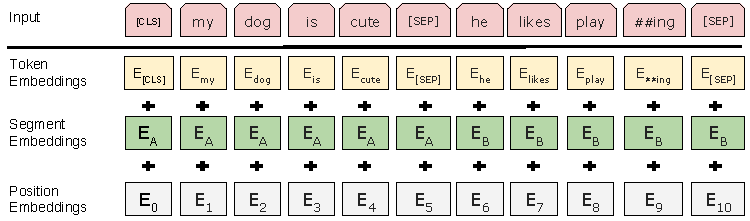
\includegraphics{figures/bert-input-representation}
\caption[BERT input representation]{BERT input representation \cite[p.~5]{devlin2018bert}}
\label{fig:bert-input-representation}
\end{figure}

Depending on the task to perform, there are different ways to use the final hidden states of the BERT Transformer network.
For sentence classification tasks, the \texttt{[CLS]} token representation can be used.
This work uses the final hidden states for every single input token, as the decoder should have access to the presentation of every input token.
For the simpler extractive summarization task, which is basically a kind of sentence classification in which each sentence is either classified as \texttt{"include in summary"} or \texttt{"do not include in summary,"} it is sufficient to only use the final hidden state of the \texttt{[CLS]} token. 
\cite{1903.10318} proposes a small input variation for BERT that inserts multiple \texttt{[CLS]} tokens into the input sequence to later use them for extractive summarization.

\paragraph{Pretraining Objectives}

BERT is pretrained with two different tasks \cite[p.~4--5]{devlin2018bert}.
For the first task, the network is given a sentence with 15\% of its WordPiece tokens randomly masked.
An example of masking is shown in \cref{fig:bert_masking_example}.

% TODO Exact source is https://github.com/google-research/bert#what-is-bert
% TODO I need to ask my prof if the current mentioning of the GitHub page is enough
\begin{figure}[h]
\begin{lstlisting}[numbers=none]
Input: the man went to the [MASK1] . he bought a [MASK2] of milk.
Labels: [MASK1] = store; [MASK2] = gallon
\end{lstlisting}
\caption[Masked input example]{Masked input example (taken from the BERT GitHub page)}
\label{fig:bert_masking_example}
\end{figure}

The task of the network is to predict the masked tokens.
This task requires the network to learn to take the context of a word into consideration.

For the second task, the network is given two sentences.
The network must then predict if the second of these two sentences comes after the first one in the original text or if it is just a randomly selected sentence from any other text.
An example of next-sentence prediction is shown in \cref{fig:bert_next_sentence_example}.

% TODO Exact source is https://github.com/google-research/bert#what-is-bert
% TODO I need to ask my prof if the current mentioning of the GitHub page is enough
\begin{figure}[h]
\begin{lstlisting}[numbers=none]
Sentence A: the man went to the store .
Sentence B: he bought a gallon of milk .
Label: IsNextSentence

Sentence A: the man went to the store .
Sentence B: penguins are flightless .
Label: NotNextSentence
\end{lstlisting}
\caption[Next-sentence prediction example]{Next-sentence prediction example (taken from the BERT GitHub page)}
\label{fig:bert_next_sentence_example}
\end{figure}

Ideally, this helps the network to understand the relationship between two sentences.
However, this task has been shown to be too simple for the network as it is easier for it to just learn if the topics of two sentences match instead of understanding the real relationship of the sentences.
To make the task harder, newer successors of BERT such as ALBERT use slightly changed training objectives, like sentence-order prediction \cite[p.~3]{1909.11942}, in which the goal is to predict which of two given sentences comes first.
This allows the network to better learn the relationship between sentences instead of just detecting matching topics.

Pretraining is usually expensive.
The training of the pretrained BERT models was performed for four days on four Cloud TPUs for BERT\textsubscript{BASE} and 16 Cloud TPUs for the larger model, BERT\textsubscript{LARGE}, with each Cloud TPU having four TPU chips \cite[p.~13]{devlin2018bert}.
However, it is only necessary to do pretraining once.

\paragraph{Fine-Tuning}

After the unsupervised pretraining, the network can be fine-tuned for a specific task.
This is done by just training a full network on the desired task for a short time.
Fine-tuning is far less expensive than pretraining and can usually be done in less than one hour on a single Cloud TPU or a few hours on a normal GPU \cite[p.~5]{devlin2018bert}.

% TODO Either summarize this chapter or lead to the next chapter

\chapter{System Description}\label{ch:system-description}

Using the knowledge from the previous chapter, this chapter first introduces the architecture of the developed neural network.
Afterward, it explains the training process together with the preparation of the training data and the overall concept to generate the final abstractive summaries.
Then it continues with a short introduction of the Texar library \cite{hu2019texar} which was used to develop the neural network.
Finally, the exact hyperparameters that were used are described.

% ===============
% MODEL ARCHITECTURE
% ===============

\section{Model Architecture}
 
\begin{figure}[h]
\centering
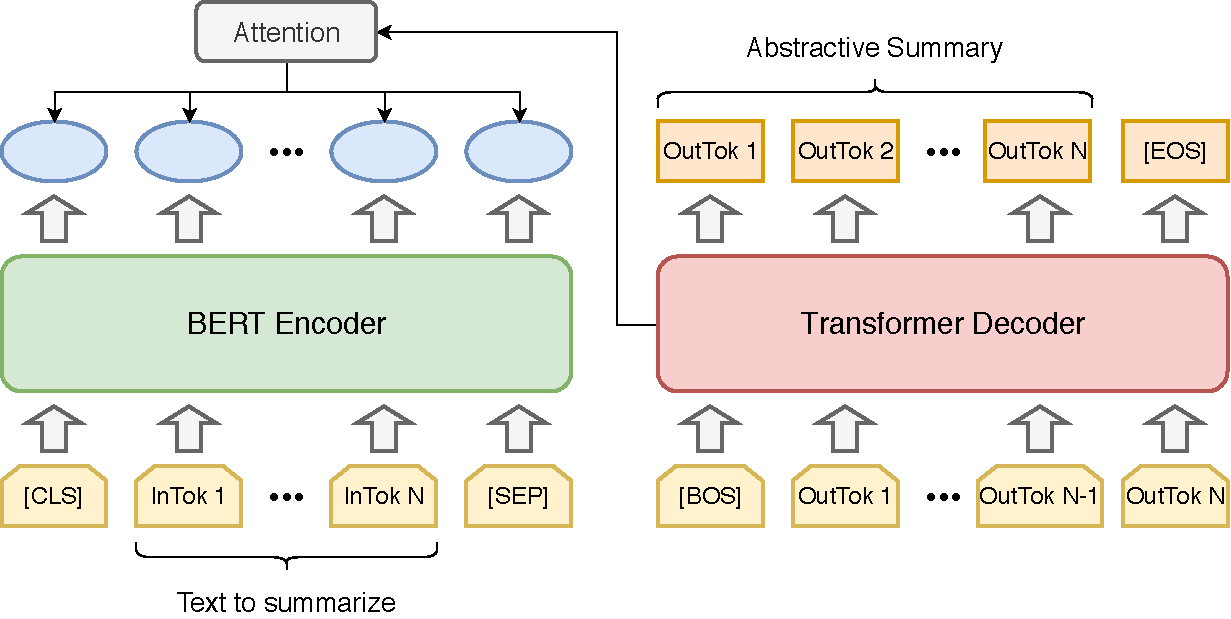
\includegraphics[width=0.7\paperwidth]{figures/summarization-architecture}
\caption{Visualization of the model architecture.}
\label{fig:summarization-architecture}
\end{figure}

The architecture of the model used in this work is rather straightforward.
For the encoding part, BERT is used, and for decoding, a normal Transformer decoder is used.
As proposed in \cite{1608.05859}, the input embeddings are tied to the output layer.

As described in \cref{sec:bert}, BERT allows either one or two sentence\footnote{It must again be noted that "sentence" is not referring to an actual linguistic sentence.} inputs.
For this work, only one sentence is used as there is no need (and logical way) to split the input into two parts.
The Transformer decoder performs attentions over the full output representations of the encoder.
The full architecture is shown in \cref{fig:summarization-architecture}.

% ================
% TRAINING AND CONCEPT
% ================

\section{Training and Concept}\label{sec:system-description-training}

% TODO I'm pretty sure that there are better examples, but for now this is fine
\begin{figure}[h]
\begin{lstlisting}[numbers=none]
DA1: Thank you very much indeed,
DA2: Cool, thank you,
DA3: So I call the meeting closed.

SUM: They close the meeting by thanking one another.
\end{lstlisting}
\caption[Three dialogue acts that are linked to one sentence of the summary]{Three dialogue acts (DA1--3) that are linked to one sentence of the summary (SUM)}
\label{fig:dialogue-arc-summary-link-example}
\end{figure}

To circumvent the high memory usage of BERT at long sequence lengths, the whole meeting transcript is not used as input for the network at once.
As described in \cref{sec:ami-meeting-corpus}, for every sentence in a meeting's abstractive summary, there exists a link to one or more dialogue acts.
These are the dialogue acts that influence the content of the sentence the most.
An example of such a link is shown in \cref{fig:dialogue-arc-summary-link-example}.
For training, all of these dialogue acts that belong to the same summary sentence are concatenated and then used as the source for the summary.
The summary sentence itself is used as the target summary.

During training, the network was evaluated on the development data set every 75 steps.
If the network improved its score, this model was saved.

To get a summary of a whole meeting, the topic segmentation described in \cref{ssec:ami-annotations} is used.
The meeting's transcript is segmented by topic, and then these segments are used as the input for the same network that was already trained to summarize dialogue acts.
Afterward, the output for all transcript segments can be concatenated.
These concatenated outputs together form the full summary of a meeting. 

\section{Preparation of the Data}\label{sec:preparation-of-the-data}

This section describes how the data of the two used corpora introduced in \cref{ch:data} is processed.

\paragraph{Format of the Corpus Data}

The corpus data for both the AMI Meeting Corpus and the ICSI Meeting Corpus is available in the NITE XML Toolkit (NXT) format \cite{Carletta2003}.
For automatic parsing, a Java library is available that makes it possible to write a Java program that traverses through the data and collects the necessary data.
For this work, such a program was developed.

It parses the data of the corpora and creates files than are easier to further process compared to the complex NXT format.
For training, three tab-separated-values (.tsv) files are created, one for each dataset (training, development, test).
For generating the final summary, it creates a text file for each meeting.
The text file contains the transcripts of the meeting split by topic, with each topic-transcript starting in a new line.
To evaluate the results, for each meeting a text file is generated that contains the summary of the meeting.

\paragraph{Data Cleaning}

In the AMI and ICSI Meeting Corpora, the transcriptions try to include every spoken word.
This includes speech disfluencies like "hmm," "huh," etc.
As these do not add any meaningful value to a sentence, they are filtered out while processing the data.
Words like "yeah," "nope," and "nah" are kept because they carry meaning, like agreement or disagreement. 

\paragraph{Data Split}

For the AMI Meeting Corpus, the recommended segmentation described in \cref{ssec:ami-segmentation-of-the-corpus} is used.
As the ISCI Meeting Corpus has no recommended segmentation, the traditional test set and a randomly generated development set are used, as described in \cref{sec:icsi-corpus}.

% ===================
% IMPLEMENTATION WITH TEXAR
% ===================

\section{Implementation with Texar}

\begin{lstlisting}[numbers=none,language=Python,caption={Hyperparameters for Transformer decoder},captionpos=b,label=lst:hyperparameters-decoder]
hidden_dim = 768

decoder = {
    'dim': hidden_dim,
    'num_blocks': 6,
    'multihead_attention': {
        'num_heads': 8,
        'output_dim': hidden_dim
    },
    'initializer': {
        'type': 'variance_scaling_initializer',
        'kwargs': {
            'scale': 1.0,
            'mode': 'fan_avg',
            'distribution': 'uniform',
        },
    },
    'poswise_feedforward': 
        tx.modules.default_transformer_poswise_net_hparams(
            output_dim=hidden_dim)
}
\end{lstlisting}

For the actual implementation of the network, the Texar toolkit \cite{hu2019texar} is used.
Texar is an open-source modular toolkit that provides plenty of useful abstractions for fast prototyping of neural network architectures with a special focus on natural language processing.
It comes in two nearly identical versions, one for TensorFlow \cite{tensorflow2015-whitepaper} and one for PyTorch \cite{NEURIPS2019_9015}.  
For this work, the TensorFlow version is used.
Texar comes with modules for both BERT and regular Transformers and allows for an easy connection of BERT and a Transformer decoder.
The code for the complete architecture is only a few hundred lines of code.
Nearly every hyperparameter, like the number of decoder layers, number of attention heads or just simple settings like the learning rate, can easily be modified.
As an example, the hyperparameter configuration for the Transformer decoder is shown in \cref{lst:hyperparameters-decoder}.

% ====================
% EXPLORING HYPERPARAMETERS
% ====================

\section{Exploring Hyperparameters}

This section explores the hyperparameters used.
The parameters were determined empirically by testing multiple variations.
After multiple tests, the following hyperparameters yielded the best results.

\begin{figure}[h]
\centering
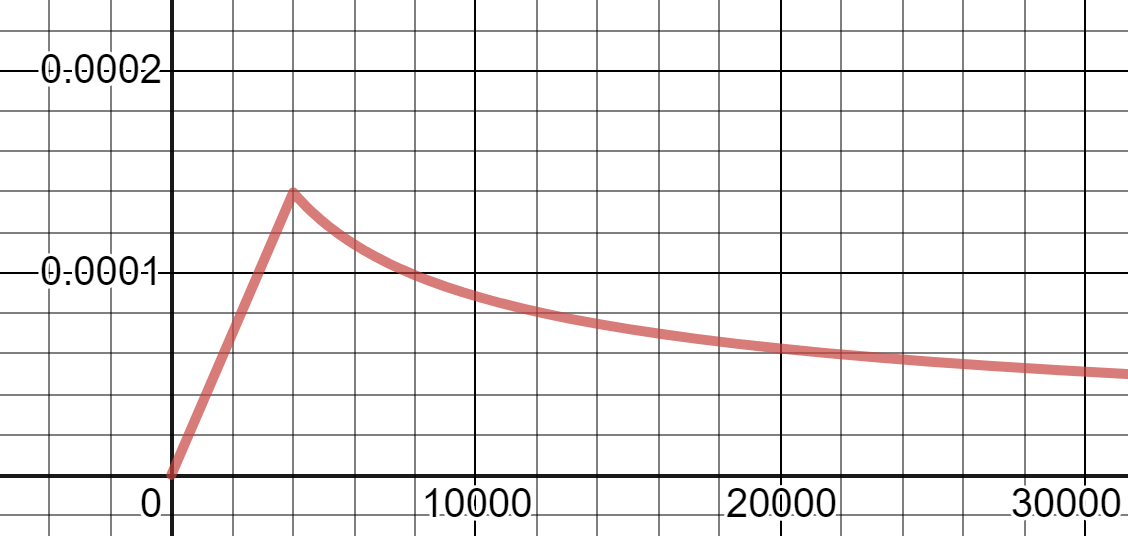
\includegraphics[width=0.6\paperwidth]{figures/learning-rate}
\caption{Visualization of the learning rate with $warmup\_steps = 4000$}
\label{fig:learning-rate}
\end{figure}

\paragraph{Optimizer and Learning Rate}

The Adam optimizer \cite{article} is used with $\beta_1=0.9$, $\beta_2=0.997$, and $\epsilon = 10^{-9}$.
The learning rate is computed by the following formula:
\[
	learning\_rate = 0.2 \cdot d_{model}^{-0.5} \cdot min(step\_num^{-0.5}, step\_num \cdot warmup\_steps^{-1.5})
\]
which is equivalent to the learning rate used to train the original Transformer \cite[p.~7]{1706.03762} but multiplied by a factor of $0.2$ because this yields better results for this training data, as shown by empirical testing.
Results for tests with a constant linear learning rate have been slightly worse.
The warmup steps are set to $warmup\_steps = 4000$.
The formula can be interpreted as linearly increasing the learning rate until $warmup\_steps < steps$ and then steadily decreasing it again.
The function's graph is visualized in \cref{fig:learning-rate}.

\paragraph{Batch Size and Maximum Sequence Length}

Due to memory constraints,\footnote{Training was performed on a single GeForce RTX 2080 Ti GPU with 11 GB of memory.} it was necessary to find a good balance between the batch size and maximum input sequence length.
For the experiments performed in this thesis, the following values proved to be a good compromise:
\begin{itemize}
\item A maximum input sequence length of $96$ % TODO Maybe provide some stats: What is the average sequence length and how many inputs were truncated with a sequence length of 96?
\item A batch size of $28$
\end{itemize}

Smaller batch sizes harm the network's performance, and smaller maximum sequence lengths mean lost information as some of the inputs are quite long and would be truncated.

\paragraph{BERT}

Due to the same memory constraints mentioned in the previous paragraph, the smaller BERT model, BERT\textsubscript{BASE}, is used as the larger model, BERT\textsubscript{LARGE}, requires significantly more memory.

\paragraph{Transformer Decoder}

For the Transformer decoder, $N=6$ stacked decoder layers are used.
The number of attention heads is set to eight, and the hidden dimension has a size of $768$, as this is the same dimension used by the BERT\textsubscript{BASE} model \cite[p.~3]{devlin2018bert}.

% TODO Concluding statement that leads to the following chapter
\chapter{Experiments}\label{ch:experiments}

Using the previously described neural network, two sets of experiments were performed.
This chapter presents the results of these experiments and the scores it achieved on the ROUGE metric.
For the second experiments, it compares the results to other summarization approaches.
It also introduces a simple baseline for better comparison.

% ==============
% INITIAL EXPERIMENTS
% ==============

\section{Initial Experiments}\label{sec:initial-experiments}

% TODO insert real data
\begin{table}[h]
\centering
\begin{tabular}{c|l|clll}
\textbf{Variant}              & \textbf{Training Steps}                                                                   & \textbf{Metric} & \textbf{Pre} & \textbf{Rec} & \textbf{F} \\ \hline
\multirow{3}{*}{\textbf{AAA}} & \multirow{3}{*}{\begin{tabular}[c]{@{}l@{}}8625 steps\\ (approx. 141 epochs)\end{tabular}} & \textbf{R-1}    & 38.49       & 29.52       & 31.92     \\
                              &                                                                                            & \textbf{R-2}    & 17.18       & 13.51       & 14.28     \\
                              &                                                                                            & \textbf{R-L}    & 34.89       & 27.01       & 26.87     \\ \hline
\multirow{3}{*}{\textbf{AAI}} & \multirow{3}{*}{\begin{tabular}[c]{@{}l@{}}8625 steps\\ (approx. 141 epochs)\end{tabular}}  & \textbf{R-1}    & 17.38         & 10.29         & 12.53       \\
                              &                                                                                            & \textbf{R-2}    & 1.14         & 0.59         & 0.76       \\
                              &                                                                                            & \textbf{R-L}    & 14.55         & 8.62         & 9.21       \\ \hline
\multirow{3}{*}{\textbf{III}} & \multirow{3}{*}{\begin{tabular}[c]{@{}l@{}}13350 steps\\ (approx. 351 epochs)\end{tabular}}  & \textbf{R-1}    & 18.48         & 14.64         & 15.55       \\
                              &                                                                                            & \textbf{R-2}    & 3.55         & 2.93         & 2.99       \\
                              &                                                                                            & \textbf{R-L}    & 15.75         & 12.44         & 12.23       \\ \hline
\multirow{3}{*}{\textbf{IIA}} & \multirow{3}{*}{\begin{tabular}[c]{@{}l@{}}13350 steps\\ (approx. 351 epochs)\end{tabular}}  & \textbf{R-1}    & 11.66         & 12.89         & 11.39       \\
                              &                                                                                            & \textbf{R-2}    & 0.61         & 0.73         & 0.63       \\
                              &                                                                                            & \textbf{R-L}    & 10.10         & 11.20         & 9.04       \\ \hline
\multirow{3}{*}{\textbf{CCC}} & \multirow{3}{*}{\begin{tabular}[c]{@{}l@{}}27000 steps\\ (approx. 270 epochs)\end{tabular}}  & \textbf{R-1}    & 32.70         & 25.28         & 27.15       \\
                              &                                                                                            & \textbf{R-2}    & 13.09         & 10.33         & 10.93       \\
                              &                                                                                            & \textbf{R-L}    & 29.28         & 22.73         & 22.45       \\ \hline
\multirow{3}{*}{\textbf{CCA}} & \multirow{3}{*}{\begin{tabular}[c]{@{}l@{}}27000 steps\\ (approx. 270 epochs)\end{tabular}}  & \textbf{R-1}    & 37.90         & 29.58         & 31.62       \\
                              &                                                                                            & \textbf{R-2}    & 17.00         & 13.40         & 14.18       \\
                              &                                                                                            & \textbf{R-L}    & 34.37         & 26.95         & 26.54       \\ \hline
\multirow{3}{*}{\textbf{CCI}} & \multirow{3}{*}{\begin{tabular}[c]{@{}l@{}}27000 steps\\ (approx. 270 epochs)\end{tabular}}  & \textbf{R-1}    & 18.68         & 13.70         & 15.13       \\
                              &                                                                                            & \textbf{R-2}    & 2.57         & 2.07         & 2.19       \\
                              &                                                                                            & \textbf{R-L}    & 15.58         & 11.38         & 11.44       \\ \hline
\end{tabular}
\caption{ROUGE scores of the initial experiments}
\label{tab:initial-experiment-rouge}
\end{table}

For the first experiments, the network is trained to summarize $n$ dialogue acts to one sentence of a meeting's abstract.
Results for the following combinations are reported:

\begin{itemize}
\item Trained on the AMI train dataset, validated on the AMI eval dataset, tested on the AMI test dataset (\textbf{AAA})
\item Trained on the AMI train dataset, validated on the AMI eval dataset, tested on the ICSI corpus (\textbf{AAI})
\item Trained on the ICSI train dataset, validated on the ICSI eval dataset, tested on the AMI test dataset (\textbf{IAA})
\item Trained, validated, and tested on the ICSI corpus, using a the split described in \cref{sec:icsi-corpus} (\textbf{III})
\item Trained, validated, and tested on a combined AMI and ICSI corpus, with all the datasets being merged with the datasets of the other corpus\footnote{\Eg the combined train set is the AMI train set + the ICSI train set} (\textbf{CCC})
\item Trained and validated on a combined AMI and ICSI corpus, tested on the AMI test data(\textbf{CCA})
\item Trained and validated on a combined AMI and ICSI corpus, tested on the AMI test data(\textbf{CCI})
\end{itemize}

All the reported results were calculated on the test set.

A single training step took, on average, about $0.41$ seconds on a single GeForce RTX 2080 Ti GPU which in turn results in a training time of about one hour for the fastest variant (AAA) and three hours for the slowest variant (CCC).
The achieved ROUGE scores are shown in \cref{tab:initial-experiment-rouge}.
While the results for AAA, CCC, and CCA are good, the network failed to generalize enough to obtain useful results for the two cross-corpus variations AAI and IAA.
The network also achieves way worse results on the more diversified ICSI Meeting Corpus compared to the AMI Meeting Corpus with its narrow scenario.
Training the network on both corpora does not improve the test results for a single corpus.

\begin{figure}[h]
\begin{lstlisting}[numbers=none]
DA: [CLS] and lea l delivered standard with a fruity colour, but
    not too not too much. but, the mai i think th the standard
    must be some kind of attractive flashy colours. so i think it
    will be a better idea to have some flashy fruity colours as as
    a standard, and for the people who really want a more
    sophisticated, more traditional look, they're willing to pay
    that. [SEP]
HS: the remote will come in fruity colours as standard with the
    option of buying different exchangeable covers.
GS: the remote will be made of fruity colors.
------------------------------------------------------------------
DA: [CLS] that's that's what i'm gonna write b between now. i'm
    going to finish my end report. [SEP]
HS: the project manager will finish the final report.
MS: the project manager will create a final report
\end{lstlisting}
\caption{Comparison between human summary (HS) and machine-generated summary (GS) of dialogue acts (DA) for variant AAA}
\label{fig:initial-experiment-example}
\end{figure}

\Cref{fig:initial-experiment-example} shows two hand-picked examples of generated summaries together with the input and the human summary.
It is easily noticeable that the network tends to overfit the data as the generated summary contains information that is not part of the actual input but can only be guessed if the settings of AMI's scenario meeting is taken into account (\eg, that the final report is always written by the project manager).
This explains the bad results for the AAI and IAA variations as the network tries to apply the setting of the AMI corpus to the ICSI corpus and vice versa.
It is also a strong indicator that more training data is necessary for the network to learn to generalize, especially considering the very specific context of the AMI scenario meetings.

However, the network is able to correctly interpret the context of a sentence and is---at least to a certain degree---able to generate new sentences.
The generated summary from the first example is not present in the training data at all but constructed from multiple different sentences.
The generated summary from the second example in \cref{fig:initial-experiment-example} is identical to a human summary that was used for training but for another input.
This human summary with the matching dialogue act in the training dataset is shown in \cref{fig:initial-experiment-training-example}.
However, the second example is the much more common case, and the network does not generate new sentences very often but only copies them from the training examples.
By reducing the number of training steps, the network tends to generate own sentences more often but at the cost of lower scores.

\begin{figure}[h]
\begin{lstlisting}[numbers=none]
DA: because I have to write the final report now.
HS: The project manager will create a final report
\end{lstlisting}
\caption{The training example, the summary of which the network copied in the second example of \cref{fig:initial-experiment-example}}
\label{fig:initial-experiment-training-example}
\end{figure}

% ================
% EXTENDED EXPERIMENTS
% ================

\section{Extended Experiments}

\begin{figure}[h]
\begin{lstlisting}[numbers=none]
the project manager gave an introduction to the goal of the
project, to create a trendy yet user-friendly remote. she
presented a long-range agenda for the whole project. the group
introduced themselves to each other and practiced with the meeting
room tools by drawing on the board. the project manager presented
the project budget, the projected price point, and the projected
profit aim for the project. then the group began a discussion
about their own experiences with remote controls to generate
initial design ideas for making the product user-friendly. they
discussed grouping features into a menu and adding an lcd display.
they also discussed the look of various materials that may be used 
n the design, in keeping with the company's goal to create
fashionable electronics. 
------------------------------------------------------------------
the group discussed making the remote universally compatible and
ergonomic design. the project manager states that the remote needs
to be original, trendy, and user - friendly. the team members then
participated in an exercise in which they drew their favorite
animals. the project manager discussed the financial goals of the
project, including the projected profit aim and price point for
the device. the team then discussed their experiences using
remotes in the past and what features to consider implementing in
the remote. the project manager closes the meeting. the marketing
expert discussed his findings from trend watching reports. the
project manager closed the meeting. 
\end{lstlisting}
\caption{Comparison of human summary (top) with machine-generated summary (bottom)}
\label{fig:extended-experiment-example}
\end{figure}

% TODO Insert real values
\begin{table}[h]
\centering
\begin{tabular}{@{}clll@{}}
\toprule
\textbf{Metric} & \multicolumn{1}{c}{\textbf{Pre}} & \multicolumn{1}{c}{\textbf{Rec}} & \multicolumn{1}{c}{\textbf{F}} \\ \midrule
\textbf{R-1}    & 36.65                           & 32.60                           & 33.54                         \\
\textbf{R-2}    & 13.68                           & 13.02                           & 12.90                         \\
\textbf{R-L}    & 33.88                           & 30.14                           & 29.44                         \\ \bottomrule
\end{tabular}
\caption{ROUGE scores of the extended experiments}
\label{tab:extended-experiment-rouge}
\end{table}

For the extended experiments, the topic segmentation described in \cref{ssec:ami-annotations} is used to split meeting transcripts into smaller pieces that are used as inputs for the same network trained in \cref{sec:initial-experiments}.
This results in one summary sentence for each topic of a meeting.
By concatenating all these summary sentences of one meeting, one can get a summary of the entire meeting.
For this experiment, only the AMI Meeting Corpus is used with the standard data split described in \cref{ssec:ami-segmentation-of-the-corpus} as there is no manual topic segmentation available for the ICSI Meeting Corpus. % TODO Maybe use the automatic segmentation with the automatic transcript?

An example of a generated summary is shown in \cref{fig:extended-experiment-example}.
The achieved ROUGE scores are shown in \cref{tab:extended-experiment-rouge}.

\paragraph{Comparison to Other Approaches}

\begin{table}[]
\centering
\begin{tabular}{@{}lcc@{}}
\toprule
                       & \textbf{R-1}     & \textbf{R-2}     \\ \midrule
\textbf{Neural (Ours)} & 33.54                & \underline{\textbf{12.90}} \\
\textbf{Ref-A}         & \underline{\textbf{37.86}} & 7.84                 \\
\textbf{Ref-B}         & 30.6                 & 6.8                  \\
\textbf{Ref-C}         & 31.5                 & 6.7                  \\
\textbf{Ref-D}         & 28.7                 & 4.2                  \\
\textbf{Baseline}      & 28.32                & 8.48                 \\ \bottomrule
\end{tabular}
\caption{Comparison of different approaches for abstractive meeting summarization and a baseline}
\label{tab:comparison}
\end{table}

The metrics used to report results are very different, and many of them are only reported for the AMI Meeting Corpus.
Some researchers only report the ROUGE-1 and ROUGE-2 scores using the F1 measure, while others also report ROUGE-L or ROUGE-SU4 scores with recall, precision, and F1 measures.
For this reason, this thesis only compares ROUGE-1 and ROUGE-2 scores using the F1 measure for the AMI corpus as these scores are reported for nearly every approach.

The results of this work's neural approach are compared to the following approaches for abstractive meeting summarization:
\begin{itemize}
\item The results from \cite{shang-etal-2018-unsupervised}, using their best-performing approach on AMI (\textbf{Ref-A})
\item The results from \cite{oya-etal-2014-template}, using their 15-segment (\textbf{Ref-B}) and 20-segment system (\textbf{Ref-C})
\item The results from \cite{mehdad-etal-2013-abstractive}, using their full model (\textbf{Ref-D})
\end{itemize}

These scores are listed in \cref{tab:comparison} together with the neural network's scores and a baseline that is described later in this section.
When just comparing the plain ROUGE scores, the neural approach achieves competitive results for ROUGE-1 scores and surpasses the ROUGE-2 scores of any of the other approaches.
However, this comparison is not fair as the other approaches only use the dialogue acts or transcripts to generate their summaries.
While this is also true for the model of this work, it has access to the abstractive summaries of the training set during its training.
Because all of AMI's scenario meetings have a very similar structure, the abstracts in the training data tend to be very similar to the abstracts in the test dataset.
This gives the network an unfair advantage over the other approaches and makes the results hardly comparable.

\begin{table}[h]
\centering
\begin{tabular}{@{}clll@{}}
\toprule
\textbf{Metric} & \multicolumn{1}{c}{\textbf{Pre}} & \multicolumn{1}{c}{\textbf{Rec}} & \multicolumn{1}{c}{\textbf{F}} \\ \midrule
\textbf{R-1}    & 26.25                           & 32.64                           & 28.32                         \\
\textbf{R-2}    & 07.88                           & 09.92                           & 08.48                         \\
\textbf{R-L}    & 23.84                           & 29.57                           & 24.40                         \\ \bottomrule
\end{tabular}
\caption{ROUGE scores of random baseline}
\label{tab:extended-experiment-rouge-random}
\end{table}

To still have a baseline that results can be compared to, one can randomly pick a summary sentence from the training data for every topic.
If the network is able to understand the meaning of its input, it should outperform this baseline.
This baseline is also included in the comparison \cref{tab:comparison}, and all scores are also shown in \cref{tab:extended-experiment-rouge-random}.
When comparing the network's scores with this baseline, the results of the network indeed outperform the baseline by a significant margin.
The fact that even this simple baseline achieves higher ROUGE-2 scores than any of the other unsupervised approaches is a clear indicator that the access to the abstracts of the training data is indeed an unfair advantage.

\paragraph{Issues with the Generated Summary}

The generated summaries come with some issues that are not visible when just looking at the ROUGE scores.
One example is duplicate sentences, or sentences that carry the same meaning, like the two sentences "The project manager closes the meeting" and "The project manager closed the meeting," which are both part of the same summary shown in \cref{fig:extended-experiment-example}.
While this issue could be solved by some clever filtering of duplicates, a more severe problem is wrong information in the summaries (\eg, the sentence "The marketing expert discussed his findings from trend watching reports" is incorrect for the meeting from \cref{fig:extended-experiment-example}).
\chapter{Outlook}\label{ch:outlook}

During the creation of this thesis, numerous new language models inspired by BERT have been released, like ALBERT \cite{1909.11942}, RoBERTa \cite{1907.11692}, and many more.
These models claim to either achieve better results or have smaller model sizes, or both.
Thus, it might be worth investigating if swapping out BERT with one of these newer models improves the results and if so, by how much.
Additionally, the larger BERT\textsubscript{LARGE} model should be tested as due to memory constraints only the smaller BERT\textsubscript{BASE} model was used in this work.
This can either be achieved by using hardware with more memory like Google's Cloud TPUs or implementing multi-GPU support.
While multiple GPUs were not supported by BERT originally, there have been many successful attempts that use Uber's Horovod \cite{sergeev2018horovod} to utilize multiple GPUs.

Another way to improve the network's performance is to find a way to give the network access to speakers' information and their roles.
Currently, only concatenated dialogue acts or the plain transcript is used as input for the neural network, but in many cases, it would be beneficial for the network to have additional information about who said which sentences.
With this information, it might generate sentences like "The project manager closed the meeting" without having to guess the information from the meeting's context.

Finally, to build a real end-to-end meeting summarizer, it is also necessary to automatically split a meeting transcript by topics.
The current topic split of AMI used in this work was created manually.
Fortunately, plenty of research on automatic topic segmentation has been conducted like \cite{10.3115/1075096.1075167}, which specifically focuses on meetings.
Such a topic segmentation algorithm can easily be applied to this work.
\chapter{Summary and Conclusion}\label{ch:summary-and-conclusion}

In this thesis, a neural approach for abstractive meeting summarization was presented.
Segmenting meeting transcripts by topics and generating a summary sentence for each of these segments proved to be a practicable solution to address the usually very long transcripts of meetings.
It was possible to generate meeting transcripts with a modest maximum sequence length of 96 using only a single GeForce RTX 2080 Ti GPU with 11GB of video memory.
The achieved ROUGE-1 scores of the presented neural approach are similar to and the achieved ROUGE-2 scores higher than any of the recent unsupervised approaches for generating abstractive summaries of meetings.
However, these results are not comparable because the neural network has an unfair advantage by having access to the summaries of the training set, while the unsupervised approaches only have the transcripts of the meetings.
To still have a baseline that can be used to validate the results, for each topic of a meeting in the test set, a random summary sentence from the training set was used.
The trained neural network achieved results that are significantly better than this simple baseline, which indicates that a neural data-driven approach seems to work.

Nonetheless, the generated summaries have several issues that make them hardly usable for practical applications.
For instance, summaries often contain duplicate or very similar sentences.
While this issue can be solved quite easily, the more significant problem involves wrong summary sentences that contain incorrect information that is not present in the input.
Additionally, cross-corpus validation shows very poor results, which indicates that utilizing transfer learning cannot compensate for the small amount of available training data.

% TODO The last line of a thesis looks to the future positively.

\backmatter
\listoffigures
\cleardoublepage

\listoftables
\cleardoublepage

\renewcommand{\lstlistlistingname}{List of Listings}  % change for German thesis
\lstlistoflistings
\cleardoublepage

\bibliographystyle{wmaainf}
\bibliography{refs}

\end{document}
